\chapter{Introduction}

\section{Our Contributions}

We propose hyper-lambda calculi.
Instead of lambda terms in ordinary lambda calculi,
we use a finite sequence of lambda terms called hyper-lambda terms.
We give two such examples:
one models synchronous send--receive communication (Chapter~\ref{ch:exchange}) and
the other models asynchronous waitfree
read--write communication (Chapter~\ref{ch:lambda}).
The two hyper-lambda calculi are in Curry--Howard correspondence with
hypersequent formulation of logics: Amida logic and G\"odel--Dummett
logic.
G\"odel--Dummett logic is an intermediate logic.
An intermediate logic is a logic \textit{between} classical and
intuitionistic logics, where `between' is defined using the
set-theoretic inclusion of valid logical formulae of each logic.
Amida logic is a substructural logic.

\citet{hosoi-ono} declared that they chose to study intermediate
logics in
general rather than studying specific intermediate logics.
However, concrete results about specific subjects matter when the
results contain new phenomena.
This thesis is intended to contain such concrete discoveries
about specific intermediate and substructural logics.

The more famous logic among the two,
G\"odel--Dummett logic, is
a typical intermediate logic logic known from 1950's.
Our method is the Curry--Howard correspondence, also known from 1940's.
Our result is characterization of waitfreedom, a concept in the theory
of distributed computation extensively studied in 1990's.
Since both sides of the correspondence is already known,
the discovery is a replay of Curry's surprise.

The less known logic, Amida logic, is our original.
After developing the hyper-lambda calculus for Amida logic,
we found that the resulting programming language is similar to one of
session type systems by \citet{giunti2010} although they were not aware
of the underlying logic.  The temporal order of discoveries is unusual
because usually logic is found first and then programming languages are
developed using Curry--Howard correspondence.  Amida logic is found
after the programming language.

We list our contributions from the most important:
\begin{enumerate}
 \item developing a lambda calculus using
       a hypersequent calculus (Chapters~\ref{ch:lambda}, \ref{ch:exchange});
 \item identifying the computational ability of the
       G\"odel--Dummett logic with waitfreedom (Chapter~\ref{ch:lambda});
 \item encoding session types using a seemingly unknown axiom
       $(\phi\limp \psi)\otimes(\psi\limp \phi)$ (which we call Amida axiom) on top
       of the multiplicative additive fragment of intuitionistic linear
       logic (Chapter~\ref{ch:exchange}),
 \item discovery of Amida logic (Chapter~\ref{ch:exchange});
 \item using conjunctive hypersequents for the first time (Chapter~\ref{ch:exchange}).
\end{enumerate}

Our first contribution is the technique for our first contribution.
We developed a lambda calculus based on \citet{avron91}'s hypersequents.
\citet{avron91} himself noted that it would be important to develop a
lambda calculus for hypersequents.
The lambda calculus relies on \citet{avron91}'s hypersequents.
The hypersequent calculus is a
variant of the deduction system called sequent calculus.  In sequent
calculus, each step of a proof tree concludes a sequent $\G\vdash\phi$ that
consists of a finite sequence of logical formulae~$\G$ and a logical
formula~$\phi$.  The sequent $\G\vdash\phi$ is
interpreted as an implication.  In hypersequent calculus, each step of a
proof tree concludes a hypersequent instead of a sequent.  A
hypersequent is a sequence of sequents delimited by $\hmid$:
$\G\vdash\phi\hmid \D\vdash\psi
\hmid \cdots$.  Also here, each component is interpreted as an
implication, and then the whole hypersequent is interpreted as the
disjunction of all those implications.
When we interpret proofs as programs, we take the components as
concurrent processeses.  Following the original disjunctive
interpretation of components, we regard the proof tree as the guarantee of
success of at least one process.

Our second contribution is finding a way to interpret proofs in
G\"odel--Dummett logic as
concurrently executable programs for waitfree computation.
Although \citet{avron91} noticed his hypersequent calculus has something
to do with concurrency (as the title of~\citep{avron91} contains the phrase
``intermediate logics for concurrency''), it was unknown that
the computational interpretation of G\"odel--Dummett logic has
the degree of synchronization called waitfreedom.  This discovery
constitutes our first contribution.

According to \citet[p.97]{curryhoward},
the Curry--Howard isomorphism~\citep{curryhoward} was first made
precise by \citet[\textbf{9}E and
\textbf{9}F]{curry1974combinatory}.
The intuitionistic propositional logic and the typed lambda calculus
had been independently invented but Curry discovered them to be the same thing.
The ``double discovery'' (\citet{wadler2012propositions}) is considered
to affirm the importance of the typed lambda calculi.
In this thesis we witness a replay of the ``double discovery'' with
different casts: G\"odel--Dummett logic and the waitfreedom.
Both of these were born in the early eras of their respective academic
disciplines:
mathematical logic bore G\"odel Dummett logic in
1950's~\citep{dummett59}
and the computer science bore waitfree computation in
1970's~\citep{lamport1979make}.
Chapter~\ref{ch:exchange} is about the unknown connection between these two.

This is the first such computational
interpretation for intermediate logics (Fig.~\ref{fig:lattice}).
Another significance of this contribution
is giving interpretation of nondterminism in typed
lambda calculi.  In the simply typed lambda calculus for intuitionistic
propositional logic, all typed terms have a unique normal form.
However, in typed lambda calculi for classical propositional logic,
there can be multiple normal forms unless we employ an evaluation
strategy or limit the set of reductions.
The lack of unique normal forms in the classical propositional proofs
has puzzled logicians for decades. \fix{mention Lafont's example; say it
is a matter of concurrency}
 \begin{figure}
  \centering
  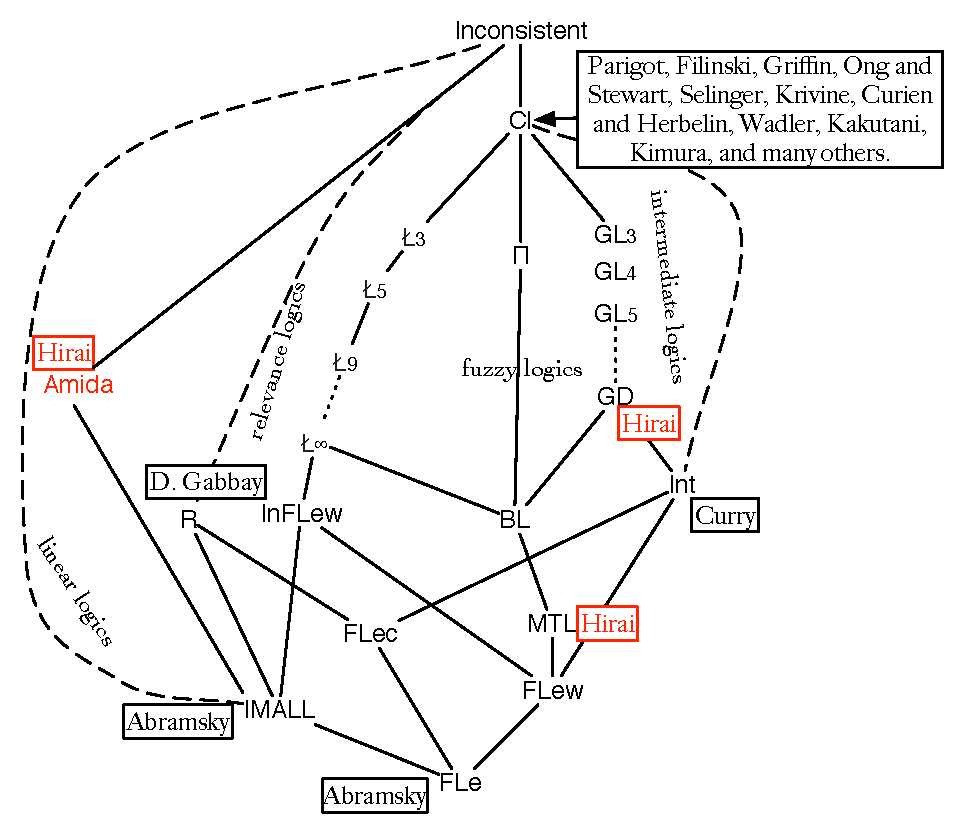
\includegraphics[scale=0.8]{lattice.eps}
  \caption[The lattice of substructural logics, some of which with known lambda calculi.]
  {The substructural logics for which lambda calculi are found.
  The underlying Hasse diagram of well-known substructural logics is
  taken from
  \cite[p.~120]{residuated} with slight modifications.
  The names in boxes refer to people who developed lambda calculi for
  these logics.
  \textsf{GD} stands for G\"odel--Dummett logic, for which
  a lambda calculus will be given in
  Chapter~\ref{ch:lambda}.
  \textsf{Amida} stands for the Amida logic, an original logic
  defined in Chapter~\ref{ch:exchange}.
  \textsf{FLe} is for the full Lambek calculus with exchange
  rule~\citep[p.86]{residuated}, which is also known as the
  intuitionistic
  multiplicative additive fragment of linear logic (IMALL).
  \textsf{MALL} stands for its classical version, the multiplicative
  additive fragment of linear logic.  For these fragments of linear
  logic,
  \citet{abramsky1993computational} gave lambda calculi.
  \textsf{FLew} stands for the full Lambek calculus with exchange and
  weakening,
  which is also known as intuitionistic affine logic.
  Affine logics lack contraction, which causes exponential size increase
  during cut-elimination process.
  Asperti gave light affine logic~\citep{asperti2002}.
  \citet{terui2007} gave an affine typed lambda calculus for polynomial
  time computation.
  \textsf{R} stands for relevance logic~\citep{urquhart1972},
  for which \citet{gabbay1992} gave a lambda calculus.
  \textsf{Int} stands for the intuitionistic propositional logic.
  The original Curry--Howard isomorphism was found for this logic by
  Curry~\citep{curry1942}.
  \textsf{Cl} stands for the classical propositional logic.
  There is intensive research going on for the computational
  interpretation of classical logic.  Namely,
  Parigot's $\lambda\mu$-calculus~\citep{lambdamu},
  Filinski's symmetric lambda calculus~\citep{filinski1989},
  Griffin's control perator~$\mathcal C$~\citep{griffin1990},
  Ong and Stewart's $\lambda\mu_{\mathrm
  v}$~\citep{ong-stewart},
%   \citet{bb1994}, this is predicate logic
  Selinger's categorical semantics and duality
  result~\citep{selinger2001} for which \citet{kakutani2002} introduced
  fixed-point
  operators,
  Curien and Herbelin's $\bar\lambda\mu\tilde\mu$
  calculus~\citep{curien2000},
  Wadler's dual calculus~\citep{wadler-dual, wadler-reloaded} and so on.
  For the history of lambda calculi for classical logic,
  Daisuke Kimura's thesis~\cite{kimura} is a source of detailed
  information.
  \textsf{Inconsistent} stands for the logic of all logical formulae.
  A programming language \texttt{Haskell}, which is based on
  the typed lambda calculi, has
  an inconsistent type system.
  }
  \label{fig:lattice}
 \end{figure}
Dynamic behaviour involves time.
One simple notion of time is that of totally-ordered events where
one event happens before the other or the other before one \fix{cite something}.
This sentence is syntactically similar to Dummett's axiom that states
one proposition implies the other or the other implies one.
We investigate whether this syntactic similarity is reflected
in the dynamic semantics of logics: namely, the lambda calculi.

Our third contribution is about encoding of session types into a linear
type system.  Although the approach is similar to \citet{pfenning2010} and
\citet{wadler2012propositions}'s work, our Amida calculus has an
additional axiom so that it can type some procsses which Pfenning or
Wadler's type systems cannot.

Our fourth contribution is a side-effect of the third contribution.
The type system we developed for our third contribution is a seemingly
unknown logic with peculiar properties.  Semantically, the falsehood is
imcompatible with Amida logic (\thref{no-falsehood}).
Syntactically, the correct proof structure can be characterized with
Amida edges, which is similar to the structure of Amida lottery.
The previous works treated the computational interpretations of
disjunctive formulae like $(\phi\imp\psi)\lor(\psi\imp\phi)$ or
$(\phi\limp\psi)\oplus(\psi\limp\phi)$.  In this chapter, we try
replacing these disjunctions with conjunctions.
In the former case, the change renders the logic inconsistent.
If we add the axiom $(\phi\imp\psi)\land(\psi\imp\phi)$ to the
intuitionistic propositional logic,
we can prove any formula.  However in the lattar case, the change does
not make the system meaningless.
In Chapter~\ref{ch:exchange}, we treat
the axioms of the form $(\phi\limp\psi)\otimes(\psi\limp\phi)$
on top of IMALL, intuitionistic
multiplicative additiver linear
logic.  In essence, the axiom allows two processes to wait for one
another and then exchange information.

Our fifth contribution is using conjunctive hypersequents.
Hypersequents have been around since \citet{avron91}, but
in all cases, different components in a hypersequent were interpreted
disjunctively.
In our formalization of Amida logic in Chapter~\ref{ch:exchange},
we use conjunctive hypersequents, where different components are
interpreted conjunctively.
This is the first application of such conjunctive hypersequents.


The content of Chapter~\ref{ch:lambda} appears in
a conference paper by the author \citep{hiraiflops2012}
although we have applied substantial modifications since then.

% \section{An Introduction for Computer Scientists}


